\chapter{Contraining neutrino magnetic moment in the NOvA near detector}\label{sec:NeutrinoMagMoment}

%%% ABSTRACT %%%

\section{Theory of neutrino magnetic moment}

\todo{Re-read the three main theory papers and double check the theoretical overview}

%Neutrino electromagnetic properties have been proposed since the very beginning by Pauli to solve the discrepancies in the electron beta emission spectra. This was solved by discovering the neutron. Then again, neutrino magnetic moment was proposed as one of the solution to the solar neutrino problem 

% Although in the standard model neutrinos are electrically neutral and do not possess electric or magnetic dipole moments, they have a charge radius which is generated by radiative corrections. [...] In many extensions of the standard model neutrinos also acquire electromagnetic properties through quantum loop effects which allow direct interactions of neutrinos with electromagnetic fields and electromagnetic interactions of neutrinos with charged particles. Hence, the theoretical and experimental study of neutrino electromagnetic interactions is a powerful tool in the search for the fundamental theory beyond the standard model. Moreover, the electromagnetic interactions of neutrinos can generate important effects, especially in astrophysical environments, where neutrinos propagate over long distances in magnetic fields in vacuum and in matter. [nuElmagInt2015.pdf]

% ...the existence of neutrino masses and mixing implies that neutrinos have magnetic moments. Since their values depend on the specific theory which extends the standard model in order to accommodate neutrino masses and mixing, experimentalists and theorists are eagerly looking for them. [nuElmagInt2015.pdf]

%Systematic theoretical studies of neutrino electromagnetic properties started after it was shown that in the extended standard model with right-handed neutrinos the magnetic moment of a massive neutrino is, in general, nonvanishing and that its value is determined by the neutrino mass (Lee and Shrock, 1977; Marciano and Sanda, 1977; Petcov, 1977; Fujikawa and Shrock, 1980; Pal and Wolfenstein, 1982; Shrock, 1982; Bilenky and Petcov, 1987). [nuElmagInt2015.pdf]

%Neutrino electromagnetic properties are important because they are directly connected to fundamentals of particle physics. For example, neutrino electromagnetic properties can be used to distinguish Dirac and Majorana neutrinos, because Dirac neutrinos can have both diagonal and off-diagonal magnetic and electric dipole moments, whereas only the off-diagonal ones are allowed for Majorana neutrinos (Schechter and Valle, 1981; Kayser, 1982, 1984; Nieves, 1982; Pal and Wolfenstein, 1982; Shrock, 1982). This is shown in detail in Secs. III.A and III.B. Another important case in which Dirac and Majorana neutrinos have quite different observable effects is the spin-flavor precession in an external magnetic field discussed in Sec. VI.B. Neutrino electromagnetic properties are also probes of new physics beyond the standard model, because in the standard model neutrinos can have only a charge radius (see Secs. III.C and VII.B). The discovery of other neutrino electromagnetic properties would be a signal of new physics beyond the standard model (Bell et al., 2005, 2006; Bell, 2007; Novales-Sanchez et al., 2008). [nuElmagInt2015.pdf]

In the Standard Model (SM), neutrinos are massless and electrically neutral particles. However, even in the SM neutrinos can have electromagnetic interaction through loop diagrams involving the charged leptons and the W boson. These interactions are described by the neutrino charge radius, described in section \ref{sec:otherNuElmagProperties} \cite{NeutrinoPropertiesSnowmass2022.pdf}.

%But this is only the neutrino charge radius, not the neutrino electric or magnetic moment (maybe also the anapole moment) "Hence, in the standard model the form factor can be interpreted as a neutrino charge radius or as an anapole moment (or as a combination of both). The standard model theory of the neutrino charge radius has a long history, with some controversies which are shortly summarized in the following." [nuElmagInt2015.pdf - sec.VIIB]

%Various theories beyond the Standard Model
To include neutrino masses required by neutrino oscillations, we must go Beyond the Standard Model (BSM), where neutrinos can acquire other electromagnetic properties \cite{nuElmagInt2015.pdf}. In the most general case, considering interactions with a single photon as shown on Fig.~\ref{fig:FeynmanNuElmagDiagram}, neutrino electromagnetic interactions can be described by an \textit{effective} interaction Hamiltonian \cite{nuElmagInt2015.pdf}
\begin{equation}
\mathcal{H}^{\left(\nu\right)}_{em}\left(x\right)=\sum^N_{k,j=1}\overline{\nu}_k\left(x\right)\Lambda^{kj}_{\mu}\nu_j\left(x\right)A^{\mu}\left(x\right).
\end{equation}
Here $\nu_k\left(x\right), k\in\left\lbrace 1,...,N\right\rbrace$ are neutrino fields in the mass basis with $N$ neutrino mass states. $\Lambda^{kj}_{\mu}$ is a general vertex function and $A^{\mu}\left(x\right)$ is the electromagnetic field.

\begin{figure}[hbtp]
\centering
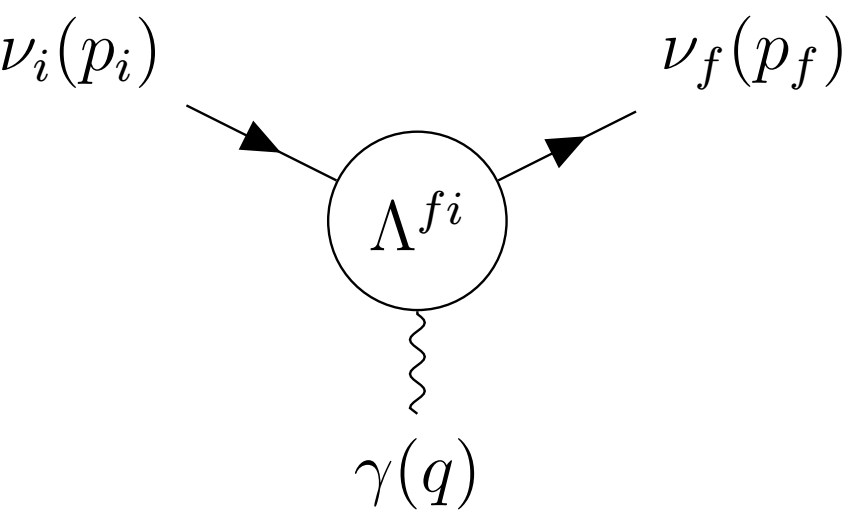
\includegraphics[width=0.4\linewidth]{Plots/NuMM/FeynmanDiagramNuElmagInt.png}
\caption{Effective coupling of neutrinos with one photon electromagnetic field 2.}
\label{fig:FeynmanNuElmagDiagram}
\end{figure}

\iffalse
The amplitude of neutrino-to-neutrino interaction for \textbf{Dirac} neutrinos is
\begin{equation}
\braket{\nu_f\left(p_f\right)|j^{\left(\nu\right)}_{\mu}\left(x\right)|\nu_i\left(p_i\right)}=
e^{i\left(p_f-p_i\right)x}\overline{u}_f\left(p_f\right)\Lambda^{fi}_{\mu}\left(p_f,p_i\right)u_i\left(p_i\right),
\end{equation}
where $p_f$ and $p_i$ are the final and initial four momentums respectively and $u/\overline{u}$ are the solutions to the Dirac equation for a free particle. We take into account possible transitions between different mass states $\nu_i$ and $\nu_f$ \cite{nuElmagInt2015.pdf}. \todo{also describe what is j}
\fi

The vertex function $\Lambda^{fi}_{\mu}\left(q\right)$ is generally a matrix and in the most general case can be written in terms of linearly independent products of Dirac matrices $\left(\gamma\right)$ and only depends on the square of the four momentum of the photon $\left(q=p_f-p_i\right)$:
\begin{align}
\Lambda^{fi}_{\mu}\left(q\right)=&
\mathbb{F}^{fi}_1\left(q^2\right)q_{\mu}+
\mathbb{F}^{fi}_2\left(q^2\right)q_{\mu}\gamma_5+
\mathbb{F}^{fi}_3\left(q^2\right)\gamma_{\mu}+
\mathbb{F}^{fi}_4\left(q^2\right)\gamma_{\mu}\gamma_5+\notag\\ &
\mathbb{F}^{fi}_5\left(q^2\right)\sigma_{\mu\nu}q^{\nu}+
\mathbb{F}^{fi}_6\left(q^2\right)\epsilon_{\mu\nu\rho\gamma}q^{\nu}\sigma^{\rho\gamma},
\end{align}
where $\mathbb{F}^{fi}_i\left(q^2\right)$ are six Lorentz invariant form factors \cite{nuElmagInt2015.pdf}.

Applying conditions of hermiticity $\left(\mathcal{H}^{\left(\nu\right)\dagger}_{em}=\mathcal{H}^{\left(\nu\right)}_{em}\right)$ and of the gauge invariance of the electromagnetic field, we can rewrite the vertex function as
\begin{equation}
\Lambda^{fi}_{\mu}\left(q\right)=
\left(\gamma_{\mu}-q_{\mu}\slashed{q}/q^2\right)\left[
\mathbb{F}^{fi}_{Q}\left(q^2\right)+\mathbb{F}^{fi}_{A}\left(q^2\right)q^2\gamma_5\right]-
i\sigma_{\mu\nu}q^{\nu}\left[\mathbb{F}^{fi}_{M}\left(q^2\right)+i\mathbb{F}^{fi}_{E}\left(q^2\right)\gamma_5\right],
\end{equation}
where $\mathbb{F}^{fi}_Q,\mathbb{F}^{fi}_M,\mathbb{F}^{fi}_E$ and $\mathbb{F}^{fi}_A$ are hermitian matrices representing the charge, dipole magnetic, dipole electric and anapole neutrino form factors. In coupling with a real photon $\left(q^2=0\right)$ these become the neutrino charge and magnetic, electric and anapole moments. The neutrino charge radius corresponds to the second term in the expansion of the charge form factor \cite{nuElmagInt2015.pdf}.

We can simplify the above expression as \cite{NeutrinoPropertiesSnowmass2022.pdf}
\begin{equation}
\Lambda^{fi}_{\mu}\left(q\right)=\gamma_{\mu}\left(Q_{\nu_{fi}}+\frac{q^2}{6}\langle r^2\rangle_{\nu_{fi}}\right)-i\sigma_{\mu\nu}q^{\nu}\mu_{\nu_{fi}},
\end{equation}
where $Q_{\nu_{fi}}$, $\langle r^2\rangle_{\nu_{fi}}$, and $\mu_{\nu_{fi}}$ are the neutrino charge, effective charge radius (also containing anapole moment), and an effective magnetic moment (also containing electric moment) respectively. This is possible thanks to the proportional effect of the neutrino charge radius and the anapole moment, or the neutrino magnetic and electric moment respectively \cite{nuElmagInt2015.pdf}. These quantities (charge, charge radius and magnetic moment) are the three neutrino electromagnetic properties measured in experiments.

\iffalse
For antineutrinos the form factors are transformed as:
\begin{equation}\label{eqAnu1}
\overline{\mathbb{F}}^{fi}_{\Omega}=-\mathbb{F}^{if}_{\Omega}=-\left(\mathbb{F}^{fi}_{\Omega}\right)^{\star} \ \ \ \Omega=Q,M,E,
\end{equation}
\begin{equation}\label{eqAnu2}
\overline{\mathbb{F}}^{fi}_{A}=\mathbb{F}^{if}_{A}=\left(\mathbb{F}^{fi}_{A}\right)^{\star}.
\end{equation}
\todo{maybe describe what does this mean?}

In case of \textbf{Majorana neutrinos}, the general expression for the vertex function in terms of charge, magnetic, electric and anapole form factors looks the same as for Dirac neutrinos.
\todo{so does that mean that the interaction amplitude can be written in the same way for both Dirac and Majorana neutrinos?} However, since Majorana antineutrinos are the same particle as Majorana neutrinos, from eq.\ref{eqAnu1},\ref{eqAnu2} we can see that:
\begin{equation}\label{eqAntisymmetryCondition}
\mathbb{F}^M_{\Omega}=-\left(\mathbb{F}^M_{\Omega}\right)^T \ \ \ \Omega=Q,M,E,
\end{equation}
\begin{equation}
\mathbb{F}^M_{A}=\left(\mathbb{F}^M_A\right)^T.
\end{equation}
Therefore the Majorana charge, magnetic and electric form factor matrices are antisymmetric and the anapole form factor matrix is symmetric. This means that Majorana neutrino doesn't have any diagonal charge and dipole magnetic and electric moments, but it can have transition  charge and magnetic and electric moment \cite{nuElmagInt2015.pdf}.
\todo{Explain why is this worth mentioning or remove it if it's not}
\fi

%%%%%%%%%%%%%%%%%%%%%%%%%%%%%%%%%%%%%%%%
\subsection{Neutrino electric and magnetic dipole moments}

The size and effect of the neutrino electromagnetic properties depends on the specific theory beyond the standard model.

Evaluating the one loop diagrams in the minimal extension of the standard model with three right handed Dirac neutrinos gives us the first approximation of the electric and magnetic moments:
\begin{equation}\label{eq:DiracMagMomExpression}
\begin{rcases}
\mu^D_{kj}\\
i\epsilon^D_{kj}
\end{rcases}
\simeq\frac{3eG_F}{16\sqrt{2}\pi^2}\left(m_k\pm m_j\right)\left(\delta_{kj}-\frac{1}{2}\sum_{l=e,\mu ,\tau}U^{\star}_{lk}U_{lj}\frac{m_l^2}{m_W^2}\right),
\end{equation}
where $m_k,m_j$ are the neutrino masses and $m_l$ are the masses of charged leptons which appear in the loop diagrams \cite{nuElmagInt2015.pdf}. $e$ is the electron charge, $G_F$ is the Fermi coupling constant, and $U$ is the PMNS neutrino oscillation matrix. Higher order electromagnetic corrections were neglected, but those can also have a significant contribution, depending on the theory.

It can be seen that there dirac neutrinos have no diagonal electric moments $\left(\epsilon_{kk}^D=0\right)$ and their diagonal magnetic moments are approximately
\begin{equation}\label{eq:DiagMagMomVal}
\mu_{kk}^D\simeq\frac{3eG_Fm_k}{8\sqrt{2}\pi^2}\simeq 3.2\times 10^{-19}\left(\frac{m_k}{\textsf{eV}}\right)\mu_B,
\end{equation}
where $\mu_B$ is the Bohr magneton \cite{nuElmagInt2015.pdf}.

The transition magnetic moments are suppressed with respect to the largest of the diagonal magnetic moments by at least a factor of $10^{-4}$ due to the $m_W^2$ in the denominator. The transition electric moments are even smaller due to the mass difference in Eq.\ref{eq:DiracMagMomExpression}. Therefore an experimental observation of a magnetic moment larger than in Eq.\ref{eq:DiagMagMomVal} would indicate physics beyond the minimally extended standard model \cite{nuElmagInt2015.pdf,nuMMMajoranaBounds2006.pdf}.

Majorana neutrinos in a minimal extension can be obtained by either adding a $\textsf{SU}\left(2\right)_L$ Higgs triplet, or right handed neutrinos together with a $\textsf{SU}\left(2\right)_L$ Higgs singlet \cite{nuElmagInt2015.pdf}. If we neglect the Feynman diagrams which depend on the model of the scalar sector, the magnetic and electric dipole moments are
\begin{equation}
\mu_{kj}^M\simeq -\frac{3ieG_F}{16\sqrt{2}\pi^2}\left(m_k+m_j\right)\sum_{l=e,\mu ,\tau}\operatorname{Im}\left[U^{\star}_{lk}U_{lj}\right]\frac{m_l^2}{m_W^2},
\end{equation}
\begin{equation}
\epsilon_{kj}^M\simeq \frac{3ieG_F}{16\sqrt{2}\pi^2}\left(m_k-m_j\right)\sum_{l=e,\mu ,\tau}\operatorname{Re}\left[U^{\star}_{lk}U_{lj}\right]\frac{m_l^2}{m_W^2}.
\end{equation}
These are difficult to compare to the Dirac case, due to possible presence of Majorana phases in the PMNS matrices, but it is clear that they have the same order of magnitude as Dirac transition dipole moments. However, the neglected model dependent contributions can enhance the transition dipole moments \cite{nuElmagInt2015.pdf}.

It is possible \cite{nuMMMajoranaBounds2006.pdf} to obtain a "natural" upper limits on the size of neutrino magnetic moment by calculating its contribution to the neutrino mass by standard model radiative corrections. For Dirac neutrinos, the radiative correction induced by neutrino magnetic moment, generated at an energy scale $\Lambda$, to the neutrino mass is generically
\begin{equation}
m_{\nu}^D\sim\frac{\mu_{\nu}^D}{3\times 10^{-15}\mu_B}\left[\Lambda\left(\textsf{TeV}\right)\right]^2\textsf{eV}.
\end{equation}
So for $\Lambda\simeq 1\textsf{TeV}$ \todo{figure out what exactly does this energy scale actually relate to and explain it here?} and $m_{\nu}\lesssim 0.3\textsf{eV}$ the limit becomes $\mu_{\nu}^D\lesssim 10^{-15}\mu_B$. This applies only if the new physics is well above the electroweak scale ($\Lambda_{EW} \sim 100\textsf{GeV}$). It is possible to get Dirac neutrino magnetic moment higher than this limit, for example in frameworks of minimal super-symmetric standard model, by adding more Higgs doublets, or by considering large extra dimensions \cite{nuElmagInt2015.pdf}.

A similar limit for Majorana neutrino magnetic moment would be less stringent due to the antisymmetry of the Majorana neutrino magnetic moment form factors. Considering $m_{\nu}\lesssim 0.3\textsf{eV}$, the limit can be expressed as 
\begin{align}
\mu_{\tau\mu},\mu_{\tau e} &\lesssim 10^{-9}\left[\Lambda\left(\textsf{TeV}\right)\right]^{-2}\\
\mu_{\mu e} &\lesssim 3\times 10^{-7}\left[\Lambda\left(\textsf{TeV}\right)\right]^{-2}
\end{align}
which is shown in the flavour basis \cite{nuMMMajoranaBounds2006.pdf}. This expression relates to the framework used previously as
\begin{equation}
\mu_{ij}=\sum_{\alpha\beta}\mu_{\alpha\beta}U^{\star}_{\alpha i}U_{\beta j},\ \ \ \alpha,\beta\in\left\lbrace e,\mu,\tau\right\rbrace.
\end{equation}

These considerations imply, that if a magnetic moment $\mu\gtrsim 10^{-15}\mu_B$ would be measured, it is more plausible that neutrinos are Majorana fermions and that the scale of lepton violation would be well below the conventional see-saw scale \cite{nuMMMajoranaBounds2006.pdf} \todo{double check this claim}.

\subsubsection{Effective neutrino magnetic moment}
Since experiments detect neutrino flavour states, not the mass states, what we measure in experiments is an effective "flavour" magnetic moment $\mu_{eff}$. $\mu_{eff}$ is influenced by mixing of the neutrino magnetic moments (and electric moments) expressed in the mass basis (as described above) and neutrino oscillations. In the ultra-relativistic limit, the (anti)neutrino effective magnetic moment is
\begin{equation}
\mu_{\nu_l}^2\left(L,E_{\nu}\right)=\sum_j\left|\sum_k U^{\star}_{lk}e^{\mp i\Delta m^2_{kj}L/2E_{\nu}}\left(\mu_{jk}-i\epsilon_{jk}\right)\right|^2,
\end{equation}
where $L$ is the distance the neutrino travelled, $E_\nu$ is the neutrino energy and $\delta m^2$ is the neutrino mass squared difference \cite{nuElmagInt2015.pdf}. The minus sign in the exponent is for neutrinos and the plus sign for antineutrinos, therefore the only difference is in the phase induced by neutrino oscillations.

For experiments with baselines short enough that neutrino oscillations would not have time to develop $\left(\Delta m^2L/2E_{\nu}\ll\sim1\right)$, such as the NOvA Near Detector, the effective magnetic moment can be expressed as
\begin{equation}
\mu_{\nu_l}^2=\mu_{\overline{\nu}_l}^2\simeq\sum_j\left|\sum_k U_{lk}^{\star}\left(\mu_{jk}-i\epsilon_{jk}\right)\right|^2=\left[U\left(\mu^2+\epsilon^2\right)U^{\dagger}+2\operatorname{Im}\left(U\mu\epsilon U^{\dagger}\right)\right]_{ll^{\prime}},
\end{equation}
which is independent of the neutrino energy and of the source to detector distance.

It is important to mention, that since the effective magnetic moment depends on the flavour of the studied neutrino, it is different (but related) for neutrino experiment studying neutrinos from different sources. Additionally some experiments, namely solar neutrino experiments, need to include matter effects on the neutrino oscillations. Therefore the reports on the value (or upper limit) of the effective neutrino magnetic moment are not directly comparable between different types of neutrino experiments. Theorists publish papers trying to extrapolate the measured effective magnetic moments to each neutrino flavour, but necessarily apply assumptions that might not hold in all BSM theories.

\subsection{Other neutrino electromagnetic properties}\label{sec:otherNuElmagProperties}
\todo{This section is not finished, most of this text is just copied from some theory papers for now}

Neutrino electric charge is heavily constraint by the measurements on the neutrality of matter (since generally neutrinos having an electric charge would also mean that neutrons have charge which would affect all heavier nuclei). It is also constrained by the SN1987A, since neutrino having an effective charge would lengthen its path through the extragalactic magnetic fields and would arrive on earth later. It can also be obtained from nu-on-e scatter from the relationship between neutrino millicharge and magnetic moment. [nuElmagInt2015.pdf - sec. VIIA]

The neutrino charge radius is determined by the second term in the expansion of the neutrino charge form factor and can be interpreted using the Fourier transform of a spherically symmetric charge distribution. It can also be negative since the charge density is not a positively defined quantity. In the SM the charge radius has the form of (possible other definitions exist)
\begin{equation}
\langle r_{\nu_l}^2\rangle_{\textsf{SM}}=\frac{G_{\textsf{F}}}{4\sqrt{2}\pi^2}\left[3-2\log\left(\frac{m_l^2}{m_W^2}\right)\right].
\end{equation}
This corresponds to $\langle r_{\nu_{\mu}}^2\langle_{\textsf{SM}}=2.4\times 10^{-33}\ \unit{cm^2}$ and similar scale for other neutrino flavours. [nuElmagInt2015.pdf - sec. VIIB]

[nuElmagInt2015.pdf - sec. VIIB]
The effect of the neutrino charge radius on the neutrino-on-electron scattering cross section is through the following shift of the vector coupling constant (Grau and Grifols, 1986; Degrassi, Sirlin, and VMarciano, 1989; Vogel and Engel, 1989; Hagiwara et al., 1994):
\begin{equation}
g_V^{\nu_l}\rightarrow g_V^{\nu_l}+\frac{2}{3}m_W^2\langle r_{\nu_l}^2\rangle\sin^2\theta_W
\end{equation}

[nuElmagInt2015.pdf - sec. VIIB]
The current experimental limits for muon neutrinos are from \todo{check the current exp. limits}  Hirsch, Nardi, and Restrepo (2003) who obtained the
following 90\% C.L. bounds on $\langle r_{\nu_\mu}^2\rangle$ from a reanalysis of
CHARM-II (Vilain et al., 1995) and CCFR (McFarland et al.,1998) data:
\begin{equation}
-0.52\times 10^{-32}<\langle r_{\nu_\mu}^2\rangle<0.68\times 10^{-32}\ \unit{cm^2}
\end{equation}

In the Standard Model, the neutrino anapole moment is somehow coupled with the neutrino charge radii and is functionally identical. the phenomenology of neutrino anapole moments is similar to that of neutrino charge radii. Hence, the limits on the neutrino charge radii discussed in Sec. VII.B also apply to the neutrino anapole moments multiplied by 6.  in the standard model the neutrino charge radius and the anapole moment are not defined separately and one can interpret arbitrarily the charge form factor as a charge radius or as an anapole moment. Therefore, the standard model values for the neutrino charge radii in Eqs. (7.35)–(7.38) can be interpreted also as values of the corresponding neutrino anapole moments. [nuElmagInt2015.pdf - sec. VIIC]

It is possible to consider  the toroidal dipole moment as a characteristic of the neutrino which is more convenient and transparent than the anapole moment for the description of T-invariant interactions with nonconservation of the P and C symmetries. the toroidal and anapole moments coincide in the static limit when the masses of the initial and final neutrino states are equal to each other. The toroidal (anapole) interactions of a Majorana as well as a Dirac neutrino are expected to contribute to the total cross section of neutrino elastic scattering off electrons, quarks, and nuclei. Because of the fact that the toroidal (anapole) interactions contribute to the helicity preserving part of the scattering of neutrinos on electrons, quarks, and nuclei, its contributions to cross sections are similar to those of the neutrino charge radius. In principle, these contributions can be probed and information about toroidal moments can be extracted in low-energy scattering experiments in the future. Different effects of the neutrino toroidal moment are discussed by Ginzburg and Tsytovich (1985), Bukina, Dubovik, and Kuznetsov (1998a, 1998b), and Dubovik and Kuznetsov (1998). In particular, it has been shown that the neutrino toroidal electromagnetic interactions can produce Cherenkov radiation of neutrinos propagating in a medium. [nuElmagInt2015.pdf - sec. VIIC]

%%%%%%%%%%%%%%%%%%%%%%%%%%%%%%%%%%%%%%%%%%%%%%%%

\subsection{Measuring neutrino magnetic moment}\label{sec:MeasuringNuMM}
The most sensitive method to measure neutrino magnetic moment is the low energy elastic scattering of (anti)neutrinos on electrons \cite{nuElmagInt2015.pdf}. The diagram for this interaction is shown on Fig.\ref{fig:NuoneDiagram} showing the two observables, the recoil electron's kinetic energy $\left(T_e=E_{e\prime}-m_e\right)$ and the recoil angle with respect to the incoming neutrino beam $\left(\theta\right)$.
\begin{figure}[hbtp]
\centering
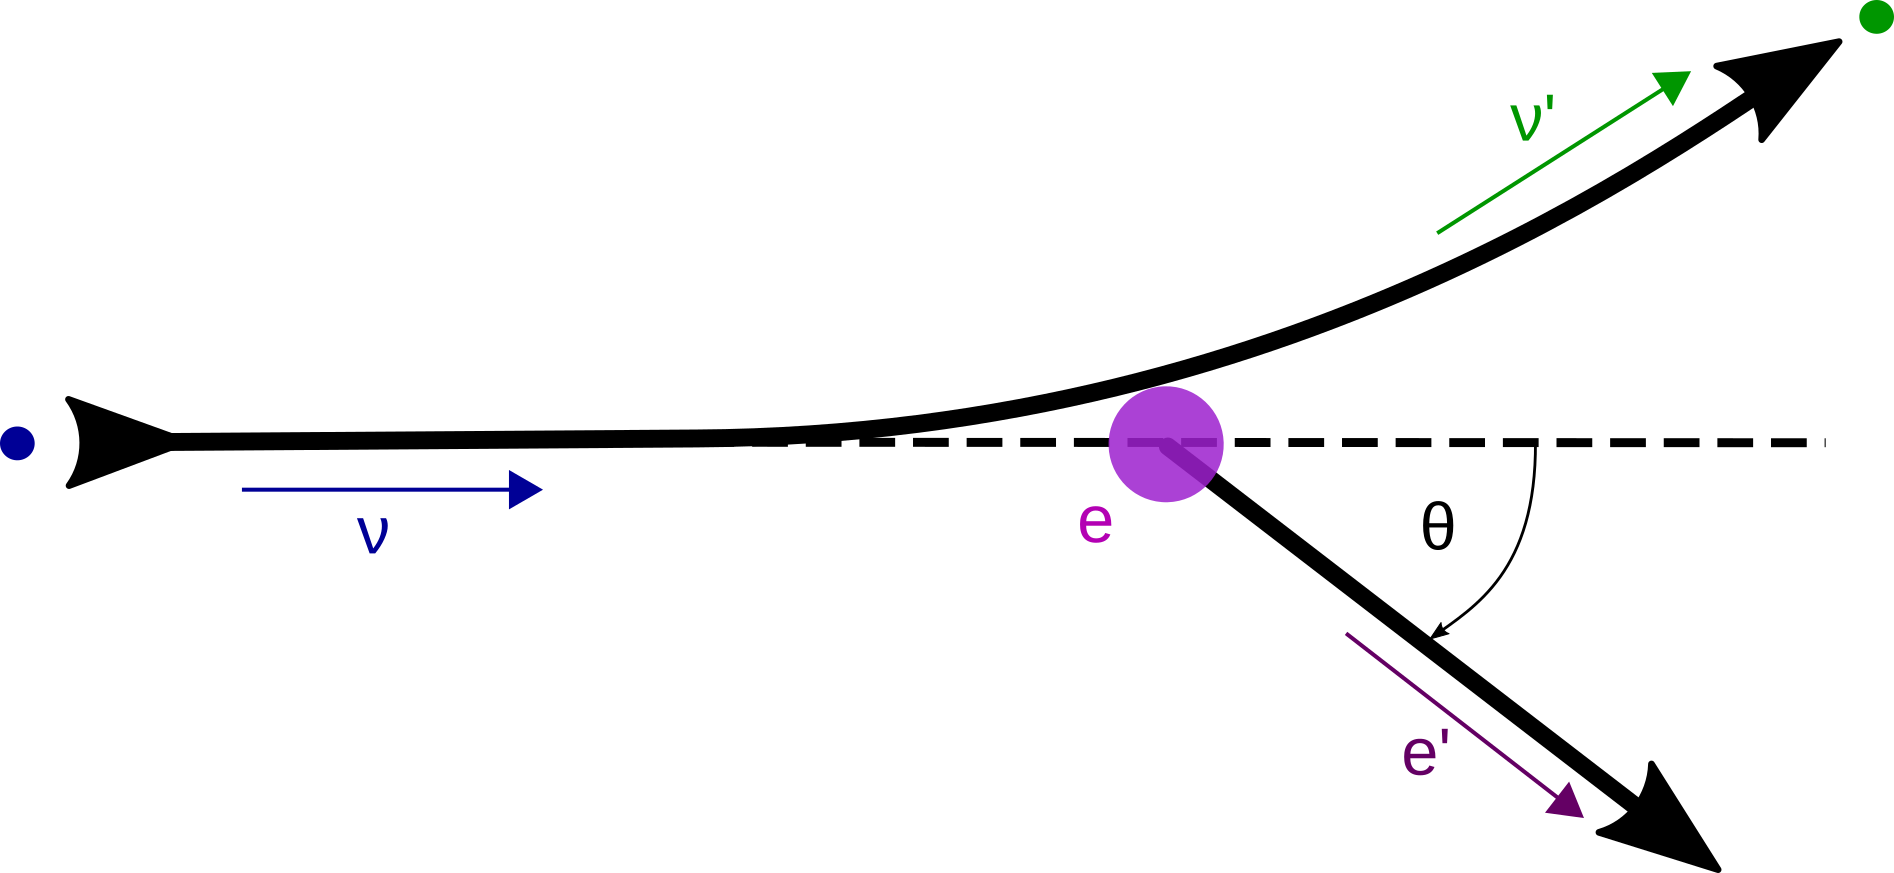
\includegraphics[width=0.55\linewidth]{Plots/NuMM/NuoneInteraction.png}
\caption{Neutrino-on-electron elastic scattering diagram}
\label{fig:NuoneDiagram}
\end{figure}

From simple $2\rightarrow 2$ kinematics we can calculate
\begin{equation}
\left(P_{\nu}-P_{e^{\prime}}\right)^2=\left(P_{\nu^{\prime}}-P_e\right)^2,
\end{equation}
\begin{equation}
m_{\nu}^2+m_e^2-2E_{\nu}E_{e^{\prime}}+2E_{\nu}p_{e^{\prime}}\cos\theta=m_{\nu}^2+m_e^2-2E_{\nu^{\prime}}m_e.
\end{equation}
Using the energy conservation
\begin{equation}
E_{\nu}+m_e=E_{\nu^{\prime}}+E_{e^{\prime}}=E_{\nu^{\prime}}+T_e+m_e\Rightarrow E_{\nu^{\prime}}=E_{\nu}-T_e
\end{equation}
we get
\begin{equation}
E_{\nu}p_{e^{\prime}}\cos\theta=E_{\nu}E_{e^{\prime}}-E_{\nu^{\prime}}m_e=E_{\nu}\left(T_e+m_e\right)-\left(E_{\nu}-T_e\right)m_e=T_e\left(E_{\nu}+m_e\right),
\end{equation}
\begin{equation}
\cos\theta=\frac{E_{\nu}+m_e}{E_{\nu}}\sqrt{\frac{T_e^2}{E_{e^{\prime}}^2-m_e^2}}=\frac{E_{\nu}+m_e}{E_{\nu}}\sqrt{\frac{T_e^2}{T_e^2+2T_em_e}}.
\end{equation}
And finally we get
\begin{equation}\label{eq:ThetaTRelation}
\cos\theta=\frac{E_{\nu}+m_e}{E_{\nu}}\sqrt{\frac{T_e}{T_e+2m_e}}.
\end{equation}

Electron's kinetic energy is kinematically constrained by the energy conservation as
\begin{equation}
T_e\leq\frac{2E_{\nu}^2}{2E_{\nu}+m_e}.
\end{equation}

Considering $E_{\nu}\sim\textsf{GeV}$, we can approximate $\frac{m_e^2}{E_{\nu}^2}\rightarrow 0$ and from Fig.\ref{fig:TThetaDistribution} we can see that we can approximate all recoil angles to be very small, therefore $\theta^2\cong \left(1-\cos^2\theta\right)$. Using Eq.\ref{eq:ThetaTRelation} we get
\begin{equation}
T_e\theta^2\cong T_e\left(1-\left(\frac{E_\nu+m_e}{E_\nu}\right)^2\frac{T_e}{T_e+2m_e}\right)
=T_e\left(1-\left(1+\frac{2m_e}{E_\nu}\right)\frac{T_e}{T_e+2m_e}\right),
\end{equation}
therefore
\begin{equation}
T_e\theta^2\cong \frac{2m_eT_e}{T_e+2m_e}\left(1-\frac{T_e}{E_\nu}\right)=2m_e\left(\frac{1}{1+\frac{2m_e}{T_e}}\right)\left(1-\frac{T_e}{E_\nu}\right),
\end{equation}
and finally
\begin{equation}\label{eqTThetaSqExp}
T_e\theta^2\cong 2m_e\left(1-\frac{T_e}{E_{\nu}}\right)<2m_e.
\end{equation}

This is a strong limit that clearly distinguishes the neutrino-on-electron elastic scattering events from other similar interaction involving single electron (mainly the $\nu_e$ Charged Current interaction).

\begin{figure}[hbtp]
\centering
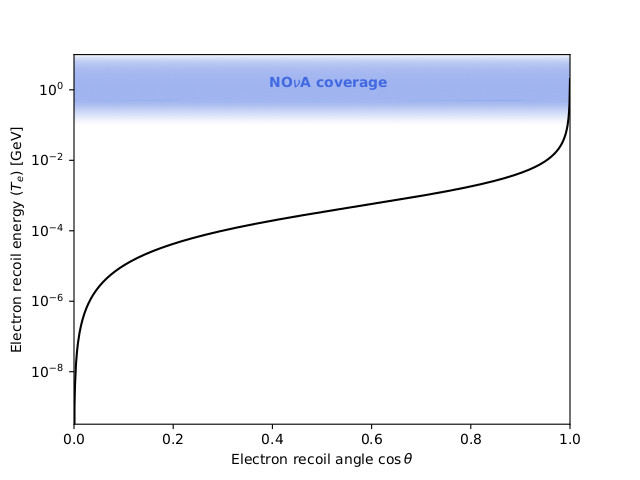
\includegraphics[width=.7\linewidth]{Plots/NuMM/KinematicsTOnTh.jpeg}
\caption{Relation between the recoil electron's kinetic energy and angle for neutrino-on-electron elastic scattering. The coverage of the NOvA detectors for measuring the electron recoil energy is shown in blue. Only very forwards electron's are recorded in NOvA.}
\label{fig:TThetaDistribution}
\end{figure}

[Fundamentals of neutrino Physics and Astrophysics, p.139]
The total neutrino-electron elastic scattering cross section for large energies is
\begin{table}{ht}
\centering
\caption{Neutrino-on-electron elastic scattering total cross sections}
\begin{tabular}{cc}
\hline
Process & Total cross section\\\hline
$\nu_e+e^-$ & $\simeq 93\times 10^{-43} E_\nu\unit{cm^2 GeV^{-1}}$\\
$\overline{\nu}_e+e^-$ & $\simeq \unit[39\times 10^{-43} E_\nu]{cm^2 GeV^{-1}}$\\
$\nu_{\mu,\tau}+e^-$ & $\simeq \unit[15\times 10^{-43} E_\nu]{cm^2 GeV^{-1}}$\\
$\overline{\nu}_{\mu,\tau}+e^-$ & $\simeq \unit[13\times 10^{-43} E_\nu]{cm^2 GeV^{-1}}$\\\hline
\end{tabular}
\end{table}


\subsubsection{Neutrino magnetic moment cross section}

In the ultrarelativistic limit, the neutrino magnetic moment changes the neutrino helicity, turning active neutrinos into sterile \todo{this is a very strong statement and it probably need a bit more backing up}. Since the SM weak interaction conserves helicity we can simply add the two contribution to the neutrino-on-electron cross section incoherently \cite{nuElmagInt2015.pdf}:
\begin{equation}
\frac{d\sigma_{\nu_le^-}}{dT_e}=\left(\frac{d\sigma_{\nu_le^-}}{dT_e}\right)_{\textsf{SM}}+\left(\frac{d\sigma_{\nu_le^-}}{dT_e}\right)_{\textsf{MAG}}.
\end{equation}

The standard model contribution can be expressed as \cite{nuElmagInt2015.pdf}:
\begin{equation}
\left(\frac{d\sigma_{\nu_le^-}}{dT_e}\right)_{\textsf{SM}}=\frac{G_F^2m_e}{2\pi}\left\lbrace\left(g_V^{\nu_l}+g_A^{\nu_l}\right)^2+\left(g_V^{\nu_l}-g_A^{\nu_l}\right)^2\left(1-\frac{T_e}{E_{\nu}}\right)^2+\left(\left(g_A^{\nu_l}\right)^2-\left(g_V^{\nu_l}\right)^2\right)\frac{m_eT_e}{E_{\nu}^2}\right\rbrace,
\end{equation}
where the coupling constants $g_V$ and $g_A$ are different for different neutrino flavours and for antineutrinos. Their values are:
\begin{align}
g_V^{\nu_e}&=2\sin^2\theta_W+1/2,\hspace{2.5cm} g_A^{\nu_e}=1/2,\\
g_V^{\nu_{\mu,\tau}}&=2\sin^2\theta_W-1/2,\hspace{2.25cm} g_A^{\nu_{\mu,\tau}}=-1/2.
\end{align}
For antineutrinos $g_A\rightarrow -g_A$.

The neutrino magnetic moment contribution is \todo{include derivation from \cite{NeutrinoElmagFormFactors1989.pdf}} \cite{nuElmagInt2015.pdf}:
\begin{equation}
\left(\frac{d\sigma_{\nu_le^-}}{dT_e}\right)_{\textsf{MAG}}=\frac{\pi\alpha^2}{m_e^2}\left(\frac{1}{T_e}-\frac{1}{E_{\nu}}\right)\left(\frac{\mu_{\nu_l}}{\mu_B}\right)^2,
\end{equation}
where $\alpha$ is the fine structure constant.

Comparison of the Standard Model and the neutrino magnetic moment cross sections is shown on Fig.\ref{fig:NuMMCrossSectionComparison}. Whereas the SM cross section is flat with $T_e\rightarrow 0$, the $\nu$MM cross section keeps increasing to infinity. However, this reach is limited by the experimental capabilities of detecting such low energetic neutrinos. Possible NOvA coverage is shown in a shaded blue and it is uncertain we could actually reach as low as $100\ \unit{MeV}$.

\todo{Reference the colours on the figures to the origins of the values (LSND and Biao)}

\begin{figure}[hbtp]
\centering
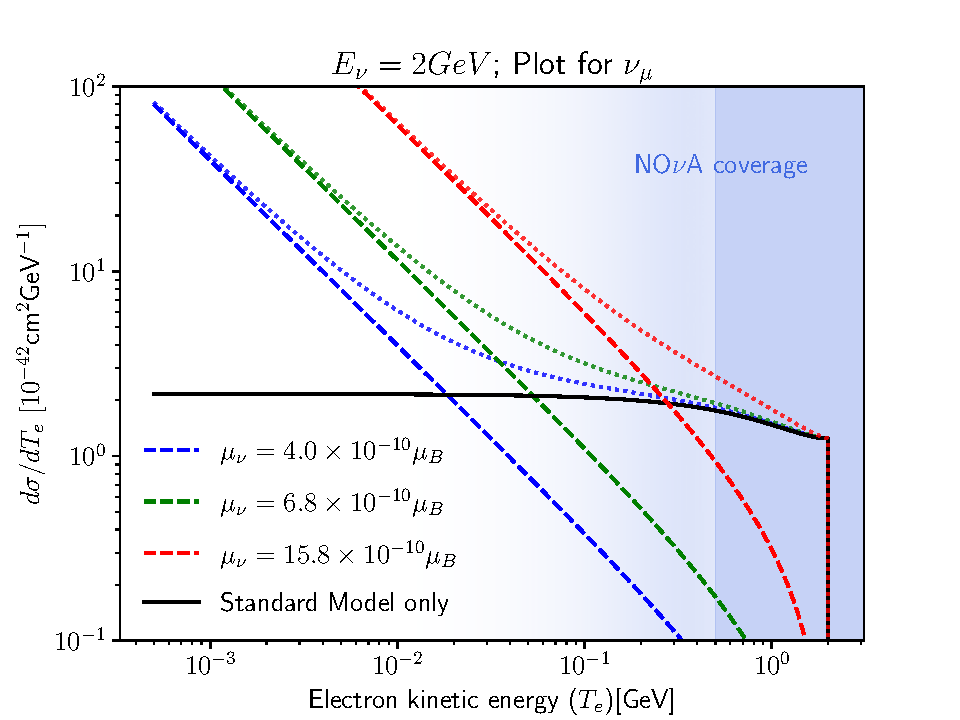
\includegraphics[width=.7\textwidth]{Plots/NuMM/dSdTNumuMMCompAltLim.pdf}
\caption{Comparison of the neutrino magnetic moment (coloured) and Standard Model (black) cross sections for the neutrino-on-electron elastic scattering. Different colours depict different values of the neutrino magnetic moment. Dashed lines are the individual cross sections and dotted lines are the added total cross section with the standard model contribution. NOvA coverage of electron recoil energies is shown in shaded blue.}
\label{fig:NuMMCrossSectionComparison}
\end{figure}

As can be seen on Fig.\ref{fig:NuMMCrossSectionComparison} and Fig.\ref{fig:NuMMCrossSectionRatios}, the magnetic moment contribution exceeds the standard model contribution for low enough $T_e$. This can be approximated as \cite{nuElmagInt2015.pdf}:
\begin{equation}
T_e\lesssim\frac{\pi^2\alpha^2}{G_F^2m_e^3}\left(\frac{\mu_{\nu}}{\mu_B}\right)^2\simeq 2.9\times 10^{19}\left(\frac{\mu_{\nu}}{\mu_B}\right)^2\left[\textsf{MeV}\right],
\end{equation}
which does not depend on the neutrino energy and makes experiments sensitive to lower energetic electrons more sensitive to the neutrino magnetic moment. This is especially true for the recent dark matter experiments which put stringent limits on the solar neutrino effective magnetic moment, as described in the following section.

\begin{figure}[hbtp]
\centering
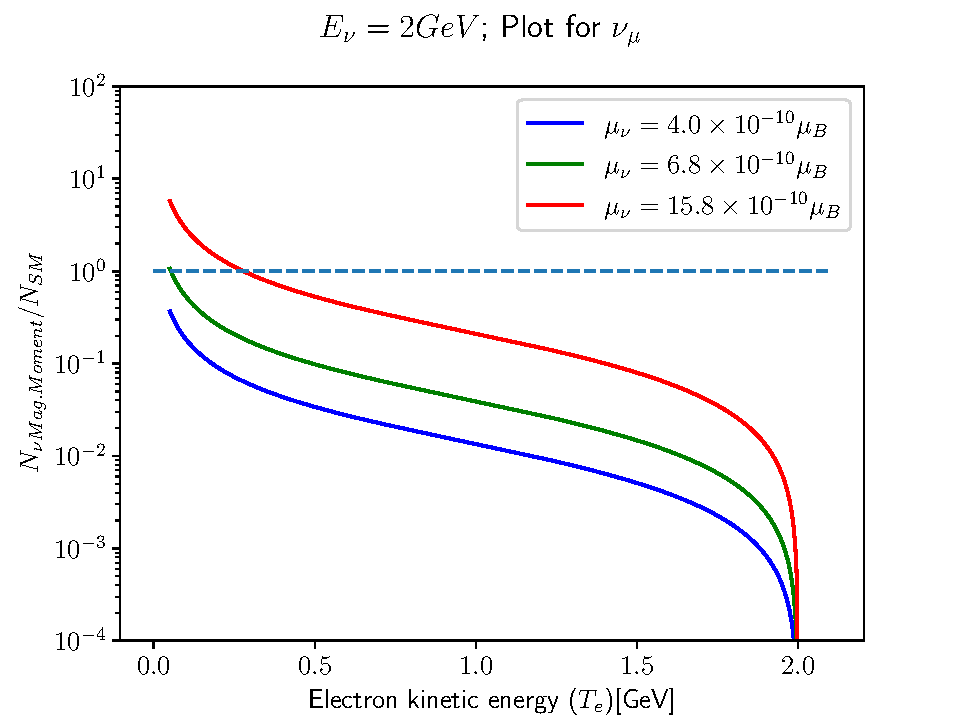
\includegraphics[width=.7\textwidth]{Plots/NuMM/RatioNumuMMCompLinX.pdf}
\caption{Ratio of the netrino magnetic moment cross section to the standard model cross section for the neutrino-on-electron elastic scattering. Different colours depict different effective muon neutrino magnetic moment values.}
\label{fig:NuMMCrossSectionRatios}
\end{figure}

%%% End of theoretical overview
%%%%%%%%%%%%%%%%%%%%%%%%%%%%%%%%%%%%%%%%%%%%%%%%%%%%%%%%%%%%%%%%%%%%%%%%%%%%%%%

\section{Experimental overview}


\section{Event selection}

\section{Fitting and hypothesis testing, parameter estimation}
How do we find the value of or limit for the effective neutrino magnetic moment?

Large section on statistics in the PDG.

Maximum likelihood with binned data:

N bins with a vector of data $n=\left(n1,...,n_N \right)$ with expectation values $\mu=E\left[n\right]$ and probabilities $f\left(n;\mu\right)$. Suppose the mean values $\mu$ can be determined as a function of a set of parameters $\theta$ (I assume for us there's either only one parameter - magnetic moment, or three parameters - mag. moment, scale of SM signal and scale of SM background). Then one may maximize the likelihood function based on the contents of the bins.

If the $n_i$ is regarded as independent and Poisson distributed (which I'd say is the case for us), then the data are instead described by a product of Poisson probabilities,
\begin{equation}
f_p\left(n;\theta\right)=\prod_{i=1}^{N} \frac{\mu_i^{n_i}}{n_i!}e^{-\mu_i},
\end{equation}
where the mean values $\mu_i$ are given functions of $\theta$. The total number of events $n_{tot}$ thus follows a Poisson distribution with mean $\mu_{tot}=\sum_i \mu_i$.

When using maximum likelihood with binned data, one can find the maximum likelihood estimators and at the same time obtain a statistic usable for a test of goodness-of-fit. Maximizing the likelihood $L\left(\theta\right)=f_P\left(n;\theta\right)$ is equivalent to maximizing the likelihood ratio $\lambda\left(\theta\right)=f_P\left(n;\theta\right) / f\left(n;\hat{\mu}\right)$, where in the denominator $f\left(n;\hat{\mu}\right)$ is a model with an adjustable parameter for each bin, $\mu=\left(\mu_1,...,\mu_N\right)$, and the corresponding estimators are $\hat{\mu}=\left(n_1,...,n_N\right)$ (called the "saturated model").

Equivalently one often minimizes the quantity $-2\ln\lambda\left(\theta\right)$. For independent Poisson distributed $n_i$ this is
\begin{equation}
-2\ln\lambda\left(\theta\right)=2\sum_{i=1}^{N}\left[\mu_i\left(\theta\right)-n_i+n_i\ln\frac{n_i}{\mu_i\left(\theta\right)}\right],
\end{equation}
where for bins with $n_i=0$, the last term is zero. In our term $\mu_i\left(\theta\right)$ is the \textbf{expected number of events in bin i if magnetic moment is $\theta$} and $n_i$ is the observed (measured) number of events in that bin.

A smaller value of $-2\ln\lambda\left(\hat{\theta}\right)$ corresponds to better agreement between the data and the hypothesized form of $\mu\left(\theta\right)$. The value of $-2\ln\lambda\left(\hat{\theta}\right)$ can thus be translated into a \textbf{p-value as a measure of goodness-of-fit}. Assuming the model is correct, then according to \textbf{Wilk's theorem}, for \textbf{sufficiently large} $\mu_i$ and provided certain regularity conditions are met, \textbf{the minimum of $-2\ln\lambda$ follows a $\chi^2$ distribution.} If there are N bins and M fitter parameters, then the number of degrees of freedom for the $\chi^2$ distribution is $N-M$ if the data are threated as Poisson distributed - which they are for us.

The method of least squares coincides with the method of maximum likelihood in a special case where the independent variables are Gaussian distributed - so I suppose this means that if I have enough events in each single bin, then I could equate the method of log likelihood and the method of least squares...

\subsection{Nuisance parameters}
In general the model is not perfect, which is to say it cannot provide an accurate description of the data even at the most optimal point of its parameter space. As a result, the estimated parameters can have a systematic bias. One can improve the model by including in it additional parameters. That is, $P\left(x|\theta\right)$ is replaced by a more general model $P\left(x|\theta,\nu\right)$, which depends on parameters of interest $\theta$ and \textit{nuisance parameters} $\nu$. The additional parameters are not of intrinsic interest but must be included for the model to be sufficiently accurate for some point in the enlarged parameter space.

Although including additional parameters may eliminate or at least reduce the effect of systematic uncertainties, their presence will result in increased statistical uncertainties for the parameters of interest. This occurs because the estimators for the nuisance parameters and those of interest will in general be correlated, which results in an enlargement of the contour.

To reduce the impact of the nuisance parameters one often tries to constrain their values by means of control or calibration measurements, say, having data \textbf{y} (I assume for us this would represent a control sample - like they use in the ND group). For example, some components of y could represent estimates of the nuisance parameters, often from separate experiments. Suppose the measurements y are statistically independent from x and are described by a model $P\left(y|\nu\right)$. The joint model for both x and y is in this case therefore the product of the probabilities for x
and y, and thus the likelihood function for the full set of parameters is
\begin{equation}
L\left(\theta,\nu\right)=P\left(x|\theta,\nu\right)P\left(y|\nu\right).
\end{equation}
Note that in this case if one wants to simulate the experiment by means of Monte Carlo, both the primary and control measurements, x and y, must be generated for each repetition under assumption of fixed values for the parameters $\theta$ and $\nu$.

Using all of the parameters $\left(\theta,\nu\right)$  to find the statistical errors in the parameters of interest $\theta$ is equivalent to using the \textit{profile likelihood}, which depends only on $\theta$. It is defined as
\begin{equation}
L_p\left(\theta\right)=L\left(\theta,\hat{\nu}\left(\theta\right)\right),
\end{equation}
This equation is supposed to have double hat for the neutrino on RHS but that throws an error when compiling...
%L\left(\theta,\hat{\hat{\nu}}\left(\theta\right)\right),
where the double-hat notation indicates the profiled values of the parameters $\nu$, defined as values that maximize $L$ for the specified $\theta$.

\subsection{Unbinned parameter estimation}
If the total number of data values is small, the unbinned maximum likelihood method is preferred, since binning can only result in a loss of information, and hence the larger statistical errors for the parameter estimates.
Does't this mean that if the number of events for the neutrino magnetic moment analysis is small, it would be better to do a completely unbinned maximum likelihood method, instead of a single bin method?


\subsection{Subsection}

\subsubsection{Subsubsection}